
%%******************************************************************************
%% SECTION -•	Métodos 
%%******************************************************************************

\subsection{Métodos}
Foram realizados dois tipos de testes com o sensor indutivo: teste de
operação e teste de comunicação via LAN.

\subsubsection{Teste de operação}
Em meados de março 2014, foram realizados testes básicos de funcionamento do
sensor indutivo. O teste consistiu em ligar o sensor em uma fonte de $15V$ e
observar o comportamento quando metais são aproximados. Foram testadas variações
de tensão entre $12V$ e $21V$, imersão do dispositivo em água e alcance do
sensoriamento aproximando metais pela lateral e pela direção alvo.

Na montagem do experimento, o sensor indutivo foi conectado ao cabo à prova
d'água M12, também da Pepperl-Fuchs. O rabicho, outra ponta do cabo, são quatro
vias com as cores marrom (alimentação do sensor), azul (GND), preta (sinal) e
branca (não conectada). O sensor indutivo apresenta LEDs que indicam o
funcionamento do dispositivo e a presença de objetos metálicos.

\subsubsection{Teste de comunicação via LAN}
O objetivo do sensor indutivo é verificar a presença de stoplogs, e com esta
análise podermos inferir se houve o contato com a garra pescadora. Dessa forma,
os dados dos sensores indutivos deverão ser enviados ao operador por rede LAN.
A saída do sensor passará por um divisor de tensão para ser regulada a 3.3V e
daí será entrada como porta GPIO de um gateway GPIO/Ethernet, que utiliza um
microcontrolador PIC. O esquema eletrônico pode ser verificado na
figura~\ref{fig:indu_banc}.

\begin{figure}[h!]
 \centering
 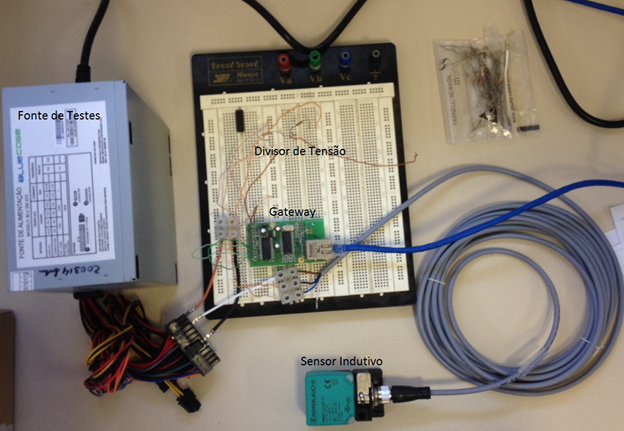
\includegraphics[width=1\columnwidth]{indutivo/figs/indutivo_bancada.png}
 \caption{Eletrônica do sensor indutivo}
 \label{fig:indu_banc}
 \end{figure}


\label{metodos}


